\section{Related Work}

The use of scientific visualization in immersive environments is simply natural, like bread and butter, while tactically important for scientific discovery, product design and data analysis. There are several high quality scientific visualization virtual reality applications that implement the applications from scratch using OpenGL directly~\cite{Billen:2008, LaViola:2007, Schulze:2001, Rantzau:1998}. These are certainly exemplary and valuable applications. However, when building immersive applications, much like desktop applications, with scientific requirements, it is often more efficient to leverage the open source visualization toolkit (VTK)~\cite{Schroeder:2004} for these development activities.

Throughout the past two plus decades, a number of research teams and developers have integrated VTK with an immersive environment to vary degrees of success. There exist three fundamental approaches to the proposed amalgamation: 

\begin{compactitem}
\item Geometry transport;
\item OpenGL context sharing; and
\item VR toolkit embedding.
\end{compactitem}

At least one additional method exists, \textit{\textbf{OpenGL intercept}}~\cite{Humphreys:2001,Humphreys:2002,Zielinski:2014,TechViz:2016,Conduit:2016}, or inserting middleware at runtime between the application and the graphics card, that enables virtual reality technologies for closed-source or proprietary applications without coding. These techniques are extremely valuable and allow scientist, engineers or medical researchers to enable their desktop applications in immersive environments with limited, but striking, interaction capabilities. Basic OpenGL, whatever that is, is sure to work using interception. But intercept methods will require more coding and tagging, if they work at all, for OpenGL 3.0+, especially when using a core OpenGL profile. In contrast to the OpenGL intercept method, the work in this paper is for the application developer, and there is no intention to eliminate the need to write code. Rather 

Our recent enhancements to the VTK platform contain solutions for the desired integration that present a number of contributions, and, therefore, we review related work for these areas.

\textbf{\textit{Geometry transport}} A historic approach to integration was the \texttt{vtkActorToPF} library~\cite{Leigh98limbo/vtk}. In this method, generation of visualization geometry is decoupled from  rendering of the geometry (see Figure~\ref{fig:vtkActorToPF}, which was recreated from Paul J. Rajlich). 

\begin{figure}[h!]
 \centering
  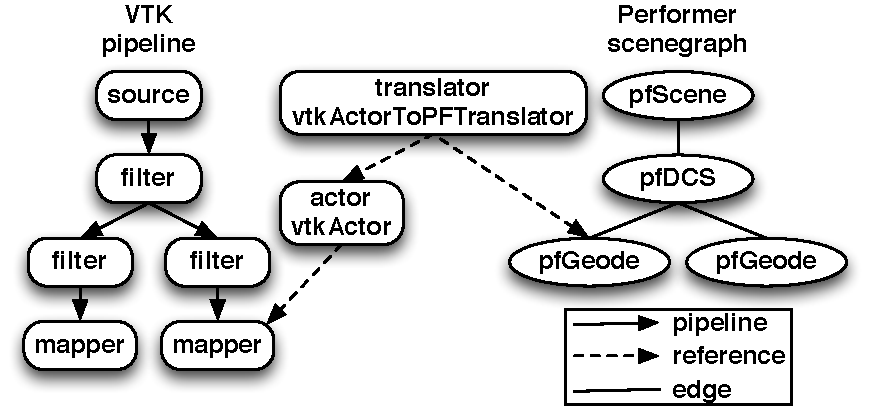
\includegraphics[width=\linewidth]{images/vtkActorToPF.pdf}
  \caption{VTK, vtkActorToPF and Performer interaction diagram.}
\label{fig:vtkActorToPF}
\end{figure}

\noindent 
VTK generates the geometry in the form of actors that consist of geometry and properties.  \texttt{vtkActorToPF} transforms these actors into pf-Geodes (nodes) that are included in a Performer (OpenSceneGraph) scene graph. The geometry is created by VTK, and the scene graph is rendered without VTK. Only geometry is transformed. Cameras, lights, rendering and interaction are not incorporated. Several applications utilized the equivalent \texttt{vtkActorToOSG} for an OpenSceneGraph-based scene graph~\cite{VE-Suite:2016} or directly into OpenGL~\cite{Ohno:2006}. Others have used VTK in a preprocessing step to produce geometries or textures eliminating the need for a direct connection to VTK\cite{Bivins:2005}.

VTK can be used to create, transport and save geometry without rendering. As effective as this approach can be, the loose coupling of VTK and a VR toolkit creates more obstacles than benefit from an application developers perspective, and is not built upon by this work.

\textbf{\textit{OpenGL context sharing}} Rather than share just the VTK geometry, the application developer would like to use all of the VTK API from within their immersive application. In VTK, the renderer and render window classes are responsible for rendering scenes. VTK creates it's own window and associates an OpenGL context with that window to be used by the renderer. An OpenGL context represents: all of the state; the default framebuffer; and everything affiliated with OpenGL with respect to the renderer, window and application. The application developer would simply like to share the OpenGL context from the VR Toolkit with a third party rendering software (e.g. Delta3D~\cite{McDowell:2006}, OpenSceneGraph~\cite{Wang:2010} and VTK). 

In previous work, by Sherman et al~\cite{Sherman:2010} and others, Delta3D and OpenSceneGraph were hacked to use the VR Toolkit's, like Vrui~\cite{Kreylos:2006}, window and associated OpenGL context. These solutions were limited in their integration. The lights, interaction and picking were not available to the application developer.

Our \texttt{vtkRenderingExternal} VTK module formalizes this integration providing lights, interaction and picking connectivity lacking in other implementations, while allowing the application developer complete access to the VTK pipeline.

\textbf{\textit{VR Toolkit embedding}} A similarly time proven approach is based on the modification of the VTK renderer and render window~\cite{van2000vista, Hannema:2001, Shamonin02vtkcave, Belleman:2003}. To render in an immersive environment, derived classes of the \texttt{Renderer} and \texttt{RenderWindow} are created, which depends on fundamental calls to the VR toolkit. Thus, VTK-based applications can simply exchanged these two items to run on the desktop or immersive environment. VTK has evolved significantly over the years, as have the diversity of virtual reality products. vtkCave~\cite{Tufo:1999}, for the CAVELib~\cite{CAVELib:2016}, followed by vjVTK~\cite{Blom:2006} and VR JuggLua~\cite{Pavlik:2012}, for VRJuggler~\cite{Bierbaum:2001}, created third party software essentially deriving RenderWindow and Renderer classes, but, from outside of VTK, lighting and interaction were not shared and/or troublesome.

In this work, we've created a new VTK module based on OpenVR~\cite{OpenVR:2016}. OpenVR is a application programming interface (API) developed by Valve for supporting  SteamVR (HTC Vive) and other virtual reality hardware~\cite{Road2VR:2015}. The OpenVR module supports several immersive environments now without the issues faced by previous work, and provides a template for embedding other VR Toolkits within VTK in the future.

\textit{\textbf{Enhanced performance}} Near real-time update of scientific visualization metaphors is crucial in these immersive environments. The field has scene several proposed solutions from decoupling rendering from processing to parallel visualization~\cite{Bryson:1996, vanReimersdahl:2000}. But here is where using VTK for scientific visualization in immersive environments really stands apart. Instead of proposed solutions in a paper and existing only in a forgotten demo, the open source, community driven VTK provides state-of-the-art implementations that are only an API call away. VTK has been around since 1993 with over one hundred thousand repository commits from over two-hundred and fifty contributors. Having the latest algorithm implementation requires using the existing implementation in VTK or contributing the it to VTK.

We present enhancements to VTK that significantly impact immersive environment application development. These enhancements include the new default OpenGL 3.2+ pipeline, dual depth peeling for transparency, and symmetric multiprocessing (SMP) tools and algorithms.